\chapter{Costos del Sistema}

 \graphicspath{{Chapter6/Figuras/}{Chapter6/Figs/PDF/}{Chapter4/Figs/}}

En este capítulo se presentan los costos del sistema de reconocimiento de estilo de conducción. Se divide en costos de componentes electrónicos y componentes mecánicos (fabricación de componentes y compra de componentes). Además se considera también un costo de envío como un 40\% del costo de los componentes. Este porcentaje representa los gastos de envío y aduanas, entre otros. Para los costos representados en dólares, se considera el valor del dólar como S/.3.39.

\section{Costos de componentes electrónicos}

Se puede observar en las Tablas \ref{diag:costos_elec_1} y \ref{diag:costos_elec_2} la lista de componentes electrónicos que conforman el sistema de reconocimiento de estilo de manejo con sus costos en dólares. Esta cotización se realizó usando DigiKey. Se muestra en la Tabla \ref{diag:costos_elec} un resumen de los costos electrónicos. Los costos en detalle y la lista de componentes se pueden encontrar en el Anexo \ref{anexo:costos}. El total es de \SI{137.75}[\$]{} ó S/.466.97

%\bgroup
%\def\arraystretch{1.5}%  1 is the default, change whatever you need
%\begin{table}[htbp!]
%\centering
%\caption{Resumen de costos electrónicos.}
%\begin{tabular}{|l|l|}
%\hline
%Item                     & Precio (\$) \\ \hline
%Componentes electrónicos & 96.39       \\ \hline
%Placa electrónica        & 2           \\ \hline
%Subtotal                 & 98.39       \\ \hline
%Envío                    & 39.36       \\ \hline
%Total                    & 137.75      \\ \hline
%\end{tabular}
%\label{diag:costos_elec}
%\end{table}
%\egroup

\begin{table}[htb!]
  \caption{Resumen de costos electrónicos}
  \label{diag:costos_elec}
  \centering
  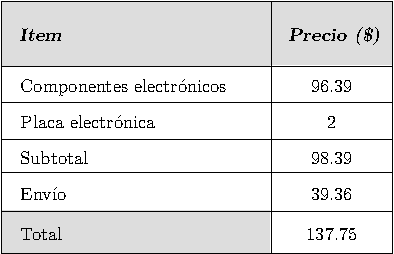
\includegraphics[width=0.55\linewidth]{costos_elec.pdf}
\end{table}


\section{Costos de fabricación y componentes mecánicos}
La Tabla \ref{diag:costos_mec} muestra los costos de fabricación del case principal y el case de la pantalla, y las piezas necesarias para el ensamble del dispositivo. La impresión 3D necesaria para el case se cotizó en 3d Print Perú, una empresa peruana de manufactura. El costo total de los componentes mecánicos es de S/.130.81.

\begin{table}[htb!]
  \caption{Resumen de costos mecánicos}
  \label{diag:costos_mec}
  \centering
  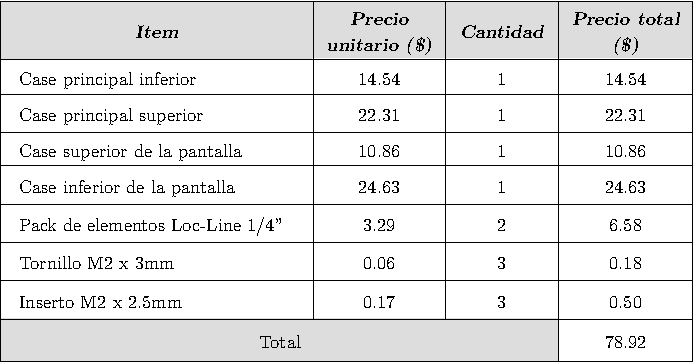
\includegraphics[width=0.9\linewidth]{costos_mec.pdf}
\end{table}

\vspace{-5mm}

\section{Costo total}
Se adiciona a los costos de los componentes electrónicos y mecánicos el costo de diseño. Se considera el costo de diseño como S/.50 por hora. Debido a que esta tesis se ha desarrollado en un tiempo de 15 semanas y en cada semana se ha invertido aproximadamente 15 horas, el costo total de diseño es S/.11847.78. El resumen de costos generales se muestra en la Tabla \ref{diag:costos_totales}.

\begin{table}[H]
  \caption{Resumen de costos totales}
  \label{diag:costos_totales}
  \centering
  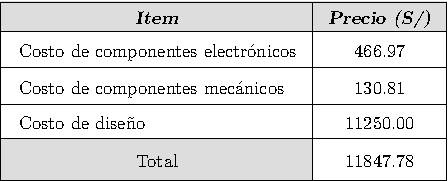
\includegraphics[width=0.6\linewidth]{costos_totales.pdf}
\end{table}
